\section{Gesamtkonzept}

Aus den morphologischen Kasten und den Nutzwertanalysen wurde folgendes Gesamtkonzept ermittelt. 

\begin{figure}[H]
\centering
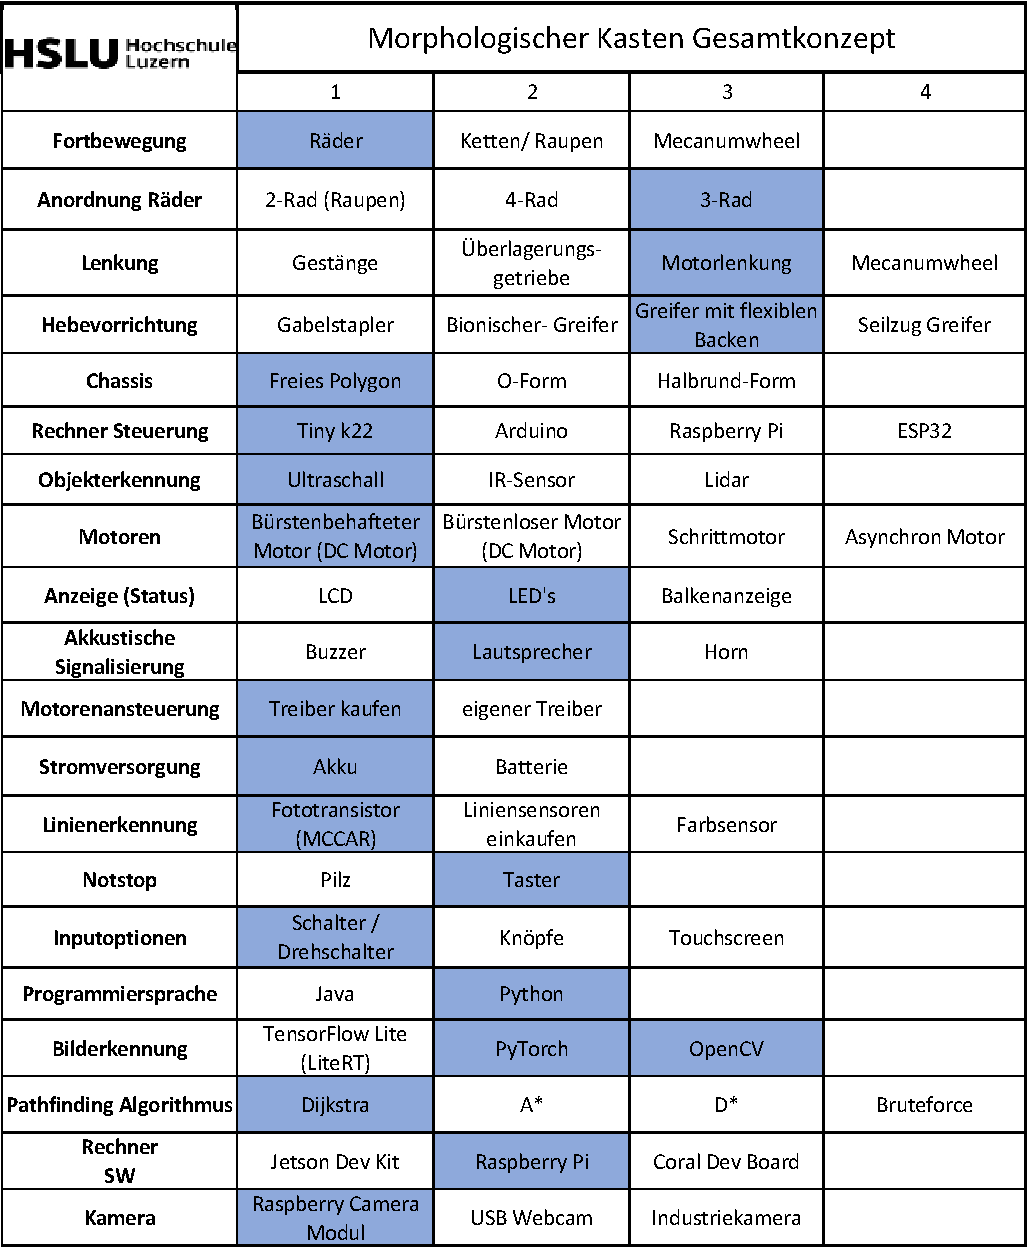
\includegraphics[width=\textwidth -40mm]{assets/MK-all.pdf}
\caption{Morphologischer Kasten}
\label{fig:mk-all}
\end{figure}

Es ist geplant einen Roboter in U-Form zu bauen, der sich mit drei Rädern fortbewegt und eine Motorlenkung besetzt. Hindernisse kann der Roboter mit einem Parallelgreifer anheben.

Die Steuerung wird auf einem Tiny k22 laufen. Die Distanz zu den Objekten wird mit Ultraschall erkannt. Die bürstebehafteten Motoren werden mit einem gekauften Treiber angesteuert. Die Stromversorgung läuft über einen Akku. Der Akkustand und der Status des Roboters wird mit LED's angezeigt. Damit der Roboter die Linien erkennt, wird ein Liniensensor mit Fototransistoren verwendet. Das Ziel wird über einen Schalter vom Benutzer ausgewählt.
Wenn der Roboter das Ziel erreicht, verkündet er dies über einen Lautsprecher. Im Notfall wird der Roboter über einen Taster ausgeschaltet.

Die Software wird in Python geschrieben und läuft auf einem Raspberry Pi. Zur Bilderkennung wird eine Kombination von PyTorch und OpenCV verwendet. Die Bilder werden mit einer Raspberry Camera aufgenommen. Der kürzeste Weg wird mit einem Dijkstra Algorithmus berechnet.

\subsection{Schnittstellen}

PLACEHOLDER

\subsection{Ablauf}

PLACEHOLDER